\documentclass[UTF8]{ctexart}
\hfuzz=4pt

\usepackage{parskip}
    \setlength{\parindent}{0em}
    \setlength{\parskip}{1em}
\usepackage{geometry}
    \geometry{left=4cm,right=4cm,top=2cm,bottom=2cm}
\usepackage{amsmath, amssymb, amsthm, mathtools}
\usepackage{thmtools}
    \renewcommand\qedsymbol{$\blacksquare$}
    \declaretheorem[numberwithin=section,shaded={rulecolor=cyan,rulewidth=2pt,bgcolor=white}]{definition}
    \declaretheorem[numberwithin=section,shaded={rulecolor=orange,rulewidth=2pt, bgcolor=white}]{theorem}
    \newtheoremstyle{mystyle}{1em plus .2 em minus .2em}{1em plus .2 em minus .2em}{}{}{\bfseries}{.}{.5em}{}
    \theoremstyle{mystyle}
    \newtheorem{axiom}{Axiom}[section]
    \newtheorem{lemma}{Lemma}[section]
    \newtheorem{proposition}{Proposition}[section]
    \newtheoremstyle{myremark}{1em plus .2 em minus .2em}{1em plus .2 em minus .2em}{}{}{\itshape}{.}{.5em}{}
    \theoremstyle{myremark}
    \newtheorem*{remark}{Remark}
    \theoremstyle{plain}
    \newtheorem{corollary}{Corollary}[section]
\usepackage{xcolor}
\usepackage{graphicx}
\usepackage{float}
\usepackage{setspace} 	 % 行间距 \begin{spacing}{arg}
\usepackage{extarrows}
\usepackage{hyperref}
    \hypersetup{colorlinks=true,linktoc=all,linkcolor=blue}
\usepackage{centernot}

    % font
\newcommand{\ve}[1]{\boldsymbol{\mathbf{#1}}}
\newcommand{\unit}[1]{\boldsymbol{\mathbf{\hat{#1}}}}
\renewcommand{\r}{\mathrm}
\renewcommand{\cal}{\mathcal}
% common symbol
\newcommand{\E}{\mathrm e}
\renewcommand{\I}{\mathrm i}
\newcommand{\R}{\mathbb R}
\newcommand{\Z}{\mathbb Z}
\newcommand{\N}{\mathbb N}
\newcommand{\Q}{\mathbb Q}
\renewcommand{\C}{\mathbb C}
\def \DD #1.#2.#3 {\dfrac{d^{#1} #2}{d #3^{#1}}}
\def \PP #1.#2.#3 {\dfrac{\partial^{#1} #2}{\partial #3^{#1}}}
\def \dd #1.#2 {\dfrac{d #1}{d #2}}
\def \pp #1.#2 {\dfrac{\partial #1}{\partial #2}} 
\newcommand{\set}[1]{\{#1\}}
\newcommand{\del}{\nabla}
\newcommand{\transp}{^{\top}}
\DeclareMathOperator{\tr}{tr}

\title{集合论}

\begin{document}
\maketitle
\tableofcontents

\newpage
注: 自然数集 $ \N $ 包含 $ 0 $.

\section{集合论基础}
我们将公理作为集合论的基础, 随后由公理逐步推到出整个集合论. 这种集合论称为公理化集合论.

\subsection{相等关系*} 
相等 ($ = $) 是一种等价关系, 需满足下面四条公理:
\begin{enumerate}
    \item 自反公理: $ x = x $
    \item 对称公理: $ x = y $ 则 $ y = x $
    \item 传递公理: $ x = y $, $ y = z $ 则 $ x = z $
    \item 代入公理: 给定两同类对象 $ x $, $ y $, 若 $ x = y $, 则对于一切函数和运算 $ f $, $ f(x) = f(y) $. 类似地, 对于任何依赖于 $ x $ 的性质 $ P(x) $, 若 $ x = y $, 则 $ P(y) $ 与 $ P(x) $ 等价.
\end{enumerate}

换句话说, 代入公理描述了: 相等的输入, 无论形式是否一样, 经过同一种运算, 应该得到相等的输出.

\paragraph{例 (代入公理)} 若 $ x = y $, 则 $ x^2 = y^2 $, $ \sin x = \sin y $, $ x + z = y + z $.

当定义一种新类型的两个对象相等时, 应该满足自反、对称和传递性; 而当定义这种类型上的新运算时, 运算应该满足代入公理, 这样定义出的运算才是良定义的 (well-defined), 否则就是病态定义的 (ill-defined).

\subsection{定义集合}
\begin{axiom}
    集合是对象的汇集, 集合本身也是对象. 
\end{axiom}

如 $ \{2, 3\} $ 是一个集合, 也是一个数学对象, 它可以是另一个集合中的元素, 例如考虑下面的集合 $ \{2, 3\} \in \{\{2, 3\}, 4, 1\} $.

\begin{remark}
    区别 $ 2 $ 和 $ \set{2} $, 两者不是同一类型的对象.
\end{remark}

\begin{definition}[\text{集合相等}]
    两个集合相等 $ A = B $ 当且仅当 $ A $ 的每个元素都是 $ B $ 的元素且 $ B $ 的每个元素都是 $ A $ 的元素.
\end{definition}

集合相等作为一种相等关系, 也是自反, 对称和传递的. 注意到: 根据集合相等的定义, 若 $ \forall x \in A $ 且 $ A = B $, 则 $ x \in B $. 意味着``属于''关系遵循代入公理. 因此我们关于集合定义的任何新运算都遵循代入律, 只要我们能纯粹使用属于 $ \in $ 来定义此运算. 本节定义的运算都是如此.

\begin{remark}
    按照定义, 两个集合相等, 集合内元素的顺序不一定相等. 集合的定义是无序的. 所以集合不存在 ``第一个元素'' 或 ``最后一个元素'' 等明显带有序性质的概念, 这样的概念违背了代入公理. 如: $ A = \{1, 2, 3 \} $, $ B = \{3, 2, 1\} $. 显然 $ A = B $. 但对于 ``$ A $ 的第一个元素是 $ 1 $'', 我们不能把 $ B $ 代入 $ A $ 得到 ``$ B $ 的第一个元素是 $ 1 $''.
\end{remark}

\subsection{构造集合}
\begin{axiom}[\text{空集}]
    存在集合 $ \varnothing $, 称为空集, 其中不含任何元素. 即对任意 $ x $, $ x \not\in \varnothing $.
\end{axiom}    

\begin{remark}
    空集亦可记为 $ \{\} $. 空集是唯一的, 意味着如果有两个空集 $ \varnothing $ 和 $ \varnothing' $, 则必然 $ \varnothing = \varnothing' $.
\end{remark}

若一个集合不是空集, 则称其为非空的. 这就引出下面的引理

\begin{lemma}[\text{单个选取}]
    若 $ A $ 非空, 则存在一个对象 $ x $ 使得 $ x \in A $.
\end{lemma}

上面引理阐述了, 如果 $ A $ 是一个非空的集合, 我们一定可以从中选取出一个元素, 证明其非空性. 这个引理后面还会逐步拓展到多个集合的选取和无穷多个集合选取的情况.

\begin{proof}
    反证法. 若 $ A $ 非空, 但找不到对象 $ x $ 使得 $ x \in A $, 也就意味着对于一切对象 $ x $, 都有 $ x \notin A $, 意味着 $ A $ 是一个空集, 矛盾. 所以一定可以找到一个对象 $ x \in A $.
\end{proof}

\begin{axiom}[\text{单元素和双元素集}]
    $ a $ 是一个对象, 则存在集合 $ \{a\} $, 它唯一的元素是 $ a $, 即对每个对象 $ y $, 有 $ y \in \{a\} $ 当且仅当 $ y = a $. 这个集合称为单元素集 (singleton).

    $ a $, $ b $ 是对象, 则存在集合 $ \{a, b\} $, 仅有的元素为 $ a $ 和 $ b $, 即对每个对象 $ y $, 有 $ y \in \{a, b\} $ 当且仅当 $ y = a $ 或 $ y = b $. 这个集合称为 $ a $ 和 $ b $ 构成的双元素集 (pair set).
\end{axiom}

\begin{remark}
    单元素集可以由双元素集定义 $ \{a\} = \{a, a\} $, 双元素集可以由单元素集和即将定义的并运算定义.
\end{remark}

\begin{definition}[\text{并运算}]
    给定两个集合 $ A $, $ B $, 存在一个集合 $ A \cup B $, 称为 $ A $ 和 $ B $ 的并, 其元素由属于 $ A $ 或属于 $ B $ 或同属两者的一切元素组成. 即对于任意对象 $ x $: \[ x \in A \cup B \Longleftrightarrow x \in A \text{ 或 } x \in B \,.\]
\end{definition}

根据代入公理, 若 $ A $, $ B $, $ A' $ 都是集合且 $ A = A' $, 则 $ A \cup B = A' \cup B $: 因为属于 $ \in $ 遵循代入公理. 

我们可以在此基础上证明 $ \cup $ 遵循交换律和结合律, 以及一些我们已经熟知的性质. 

\begin{remark}
    设 $ A $, $ B $ 为任意集合. 若 $ x \in A $, 那么 $ x \in A $ 或 $ x \in B $ 的命题就是真的, 这意味着也有 $ x \in A \cup B $.
\end{remark}

\begin{proposition}
    $ A \cup \varnothing = A $, 即 $ \varnothing $ 是并运算的单位元.
\end{proposition}

\begin{proof}
    设 $ x \in A \cup \varnothing $, 按照并运算的定义, $ x \in A $ 或 $ x \in \varnothing $. 按照空集的定义, $ x \in \varnothing $, 所以 $ x \in A $. 设 $ x \in A $, 按照并运算的定义, $ x \in A \cup \varnothing $. 综上所述, $ A \cup \varnothing $ 中的所有元素都在 $ A $ 中, $ A $ 中的所有元素都在 $ A \cup \varnothing $ 中. 故 $ A \cup \varnothing = A $.
\end{proof}


\begin{proposition} \ 
    \begin{enumerate}
        \item 并运算是交换的: $ A \cup B = B \cup A $
        \item 并运算是结合的: $ (A \cup B) \cup C = A \cup (B \cup C) $
        \item 幂等律: $ A \cup A = A $
    \end{enumerate}
\end{proposition}

\begin{proof}[\text{证明并运算是结合的}]
    设 $ A $, $ B $, $ C $ 为任意集合. 设 $ x \in (A \cup B) \cup C $, 按照定义, $ x \in A \cup B $ 或 $ x \in C $. 若 $ x \in C $, 则按照定义 $ x \in B \cup C $, 也就有 $ x \in A \cup (B \cup C) $; 若 $ x \in A \cup B $, 则 $ x \in A $ 或 $ x \in B $, 而 $ x \in A \Longrightarrow x \in A \cup (B \cup C) $, $ x \in B \Longrightarrow x \in B \cup C \Longrightarrow x \in A \cup (B \cup C) $. 所以若 $ x \in (A \cup B) \cup C $, $ x \in A \cup (B \cup C) $.

    现设 $ x \in A \cup (B \cup C) $, 按照定义, $ x \in A $ 或 $ x \in B \cup C $. 若 $ x \in A $, 则 $ x \in A \cup B $, 也就有 $ x \in (A \cup B) \cup C $; 若 $ x \in B \cup C $, 则 $ x \in B $ 或 $ x \in C $, 而 $ x \in B \Longrightarrow x \in A \cup B \Longrightarrow x \in (A \cup B) \cup C $, $ x \in C \Longrightarrow x \in (A \cup B) \cup C $. 所以若 $ x \in A \cup (B \cup C) $, 则 $ x \in (A \cup B) \cup C $.

    故 $ (A \cup B) \cup C $ 的所有元素在 $ A \cup (B \cup C) $ 中, $ A \cup (B \cup C) $ 的所有元素在 $ (A \cup B) \cup C $ 中. 按照定义 $ (A \cup B) \cup C = A \cup (B \cup C) $.
\end{proof}

由于存在结合律, $ A \cup B \cup C $ 的写法含义就明确了.


\subsection{子集}
\begin{definition}[\text{子集}]
    $ A $, $ B $ 是集合. 称 $ A $ 是 $ B $ 的子集, 记作 $ A \subseteq B $, 当且仅当 $ A $ 的每个元素都是 $ B $ 的元素, 即 \[ \forall x \in A \Longrightarrow x \in B \,.\]

    称 $ A $ 是 $ B $ 的真子集, 记作 $ A \subset B $, 如果 $ A \subseteq B $ 且 $ A \neq B $. 
\end{definition}

集合的包含关系就犹如数的 $ \leqslant $ 和 $ < $. 集合的包含也部分安排了序

\begin{remark}
    给定两个不同的自然数, 其中一个必然小于另一个. 但给定两个不同的集合, 其中一个不一定是另一个的子集. 所以说集合被部分安排了次序, 而自然数被完全安排了次序.
\end{remark}

\begin{proposition}[\text{子集性质}]
    设 $ A $, $ B $, $ C $ 为集合. 
    \begin{enumerate}
        \item 自反: $ A \subseteq A $
        \item 反对称: $ A \subseteq B $ 且 $ B \subseteq A $ $ \Longleftrightarrow $ $ A = B $
        \item 传递: 若 $ A \subseteq B $, $ B \subseteq C $ 则 $ A \subseteq C $
    \end{enumerate}
\end{proposition}

\begin{proposition}[\text{真子集性质}]
    设 $ A $, $ B $, $ C $ 为集合. 
    \begin{enumerate}
        \item 非自反: $ A \not\subset A $
        \item 非对称: $ A \subset B \centernot \Longrightarrow B \subset A $ 
        \item 传递: 若 $ A \subset B $, $ B \subset C $ 则 $ A \subset C $
    \end{enumerate}
\end{proposition}

子集的反对称性是证明集合相等的常用方法.

同样, 子集也遵循代入公理: $ A \subseteq B $, $ A = A' $, $ B = B' $, 则 $ A' \subseteq B $ 以及 $ A \subseteq B' $.

\begin{axiom}[\text{分类公理}]
    设 $ A $ 是一个集合, $ \forall x \in A $, 设 $ P(x) $ 为一个关于 $ x $ 的性质(命题). 那么存在一个集合 $ \{ x \in A \mid P(x) \text{ 成立} \} $ 或简写为 $ \{ x \in A \mid P(x) \} $, 表示 $ A $ 中满足 $ P(x) $ (使 $ P(x) $ 成立) 的元素的集合. 即对任意对象 $ y $, \[ y \in \{x \in A \mid P(x)\} \Longleftrightarrow y \in A \text{ 且 } P(y) \text{ 成立} \,.\]
\end{axiom}

这个公理通过一个命题 $ P(x) $, 使得我们从原集合中构造出子集合. 

\paragraph{例} 设关于 $ x $ 的命题 $ P(x) $ 代表 $ x < 3 $. 则对于集合 $ \set{1, 2, 3, 4, 5} $, 应用分类公理, 可得到集合 $ \set{x \in A \mid P(x)} = \set{x \in A \mid x < 3} = \set{1, 2} $.

\paragraph{例} 设命题 $ P(x) $: 存在 $ y \in \Z $, 使得 $ y^2 = x $. 即 $ P(x) $ 表示 $ x $ 是一个平方数. 则对集合 $ \set{1, 2, 3, 4, 5} $ 应用分类公理, 可以得到集合 $ \set{x \in A \mid P(x)} = \set{x \in A \mid \exists y \in \Z, y^2 = x} = \set{1, 4} $.

使用分类公理, 可以容易地定义交集.

\begin{definition}[\text{交}]
    给定两个集合 $ A $, $ B $, 定义其交集 $ A \cap B $ 为
    \[ A \cap B \coloneqq \{x \in A \mid x \in B\} \,.\]

    换句话说, 就是既属于 $ A $ 又属于 $ B $ 的元素构成的集合.
\end{definition}

\begin{proposition}
    $ A \cap \varnothing = \varnothing $, 即 $ \varnothing $ 是交运算的零元.
\end{proposition}

\begin{proof}
    反证法. 设 $ A \cap \varnothing $ 非空, 则根据单个选择公理, 可以从中选择出一个元素, 证明其非空性. 所以可以找到 $ x \in A \cap \varnothing $. 根据交集定义, 需要同时有 $ x \in A $ 和 $ x \in \varnothing $, 而这与空集的定义相违背, 因为不存在 $ x \in \varnothing $.
\end{proof}

\begin{proposition} \ 
    \begin{enumerate}
        \item 交运算是交换的: $ A \cap B = B \cap A $
        \item 交运算是结合的: $ (A \cap B) \cap C = A \cap (B \cap C) $
        \item 幂等律: $ A \cap A = A $
    \end{enumerate}
\end{proposition}

\begin{proposition} \ 
    \begin{enumerate}
        \item 并对交有分配律: \[ A \cup (B \cap C) = (A \cup B) \cap (A \cup C) \] \[ (A \cap B) \cup C = (A \cup C) \cap (B \cup C) \]
        \item 交对并有分配律: \[ A \cap (B \cup C) = (A \cap B) \cup (A \cap C) \] \[ (A \cup B) \cap C = (A \cap C) \cup (B \cap C) \]
        \item 吸收律: \[ A \cup (A \cap B) = A \] \[ A \cap (A \cup B) = A \]
    \end{enumerate}
\end{proposition}

\begin{proof}
    此处证明左分配律, 右分配律可以由交换律和左分配律推出.

    (1) 对于任意 $ x \in A \cup (B \cap C) $, 按照并定义 $ x \in A $ 或 $ x \in B \cap C $. 当 $ x \in A $ 时, $ x \in A \cup B $, 也有 $ x \in A \cup C $. 所以 $ x $ 同时属于 $ A \cup B $ 和 $ A \cup C $, $ x \in (A \cup B) \cap (A \cup C) $. 当 $ x \in B \cap C $ 时, $ x \in B $ 且 $ x \in C $. 由于 $ x \in B $, $ x \in A \cup B $; 由于 $ x \in C $, $ x \in A \cup C $. 所以同时有 $ x \in A \cup B $ 和 $ x \in A \cup C $. 以上说明了: $ A \cup (B \cap C) \subseteq (A \cup B) \cap (A \cup C) $.

    对于任意 $ x \in (A \cup B) \cap (A \cup C) $, $ x \in A \cup B $ 和 $ x \in A \cup C $ 要同时满足. 我们可以考虑两种情况, 任意 $ x \in A $ 或 $ x \notin A $. 若 $ x \in A $, 则 $ x \in A \cup (B \cap C) $; 若 $ x \notin A $, 由于 $ x \in A \cup B $ 且 $ x \in A \cup C $, 所以 $ x \in B $ 且 $ x \in C $, 即 $ x \in B \cap C $, 所以 $ x \in A \cup (B \cap C) $. 以上说明了: $ (A \cup B) \cap (A \cup C) \subseteq A \cup (B \cap C) $.

    综上所述: $ (A \cup B) \cap (A \cup C) = A \cup (B \cap C) $.

    (2) 对于任意 $ x \in A \cap (B \cup C) $, $ x \in A $ 且 $ x \in B \cup C $. 当 $ x \in B $ 时, 由于同时有 $ x \in A $, 故 $ x \in A \cap B $, 也就有 $ x \in (A \cap B) \cup (A \cup C) $; 当 $ x \in C $ 时, 同理有 $ x \in A \cap C $, 也就有 $ x \in (A \cap B) \cup (A \cup C) $. 以上说明了: $ A \cap (B \cup C) \subseteq (A \cap B) \cup (A \cap C) $.

    而对于任意 $ x \in (A \cap B) \cup (A \cap C) $, $ x \in A \cap B $ 或 $ x \in A \cap C $. 当 $ x \in A \cap B $ 时, $ x \in A $ 且 $ x \in B $, 故 $ x \in A $ 且 $ x \in B \cup C $, 即 $ x \in A \cap (B \cup C) $; 当 $ x \in A \cap C $ 时, $ x \in A $ 且 $ x \in C $, 故 $ x \in A $ 且 $ x \in B \cup C $, 即 $ x \in A \cap (B \cup C) $. 以上说明了: $ x \in A \cap (B \cup C) $.

    综上所述: $ A \cap (B \cup C) = (A \cap B) \cup (A \cap C) $.

    (3) 设 $ x \in A \cup (A \cap B) $, 则 $ x \in A $ 或 $ x \in A \cap B $. 当 $ x \in A $ 时, 直接推出, $ A \cup (A \cap B) \subseteq A $. 当 $ x \in A \cap B $ 时, $ x \in A $ 且 $ x \in B $. 所以 $ x \in A $ 成立, $ A \cup (A \cap B) \subseteq A $. 以上说明了: $ A \cup (A \cap B) \subseteq A $. 

    现设 $ x \in A $, 显然有 $ x \in A \cup (A \cap B) $. 这说明了 $ A \subseteq A \cup (A \cap B) $.

    综上所述: $ A \cup (A \cap B) = A $.

    对于 $ A \cap (A \cup B) = A $ 的证明, 方法基本和上面类似, 此处省略.
\end{proof}

\begin{definition}[\text{差}]
    给定两个集合 $ A $ 和 $ B $. 定义 $ A $ 减去 $ B $:
    \[ A \setminus B = \{x \in A \mid x \not\in B\} \,.\]
\end{definition}

\begin{proposition}
    设 $ A \subseteq X $, $ B \subseteq X $: 
    \begin{enumerate}
        \item 最大元: \[ A \cup X = X \] \[ A \cap X = A \]
        \item 分拆法: \[ X \cup (X \setminus A) = X \] \[ X \cap (X \setminus A) = \varnothing \]
        \item De Morgan 律: \[ X \setminus (A \cup B) = (X \setminus A) \cap (X \setminus B) \] \[ X \setminus (A \cap B) = (X \setminus A) \cup (X \setminus B) \]
    \end{enumerate}
\end{proposition}

\begin{remark}
    通过结合律以及归纳法, De Morgan 律可推广到多个集合的并/交的补. 即: \[ X \setminus (A_1 \cup \cdots \cup A_n) = (X \setminus A_1) \cap \cdots \cap (X \setminus A_n) \] \[ X \setminus (A_1 \cap \cdots \cap A_n) = (X \setminus A_1) \cup \cdots \cup (X \setminus A_n) \]
\end{remark}
    



\begin{axiom}[\text{替换公理}]
    给定一个集合 $ A $, 对于所有 $ x \in A $ 和任意对象 $ y $ 有命题 $ P(x, y) $. 如果对于所有 $ x \in A $, 存在最多一个 $ y $ 满足 $ P(x, y) $, 则可以构造集合 $ \{ y \mid \text{某 } x \in A \text{ 满足 } P(x, y) \} $.
\end{axiom}

替换公理采用某种规则 $ P(x, y) $, 将 $ A $ 中的部分元素 $ x $ 替换为另一个元素 $ y $, 这些替换后的元素组成新的集合.

\paragraph{例} 
集合 $ A = \{2, 3, 4\} $, 经替换公理 $ B = \{y \mid \text{某 } x \in A \text{ 满足 } y = x^2 \} $, 得到的 $ B = \{4, 9, 16\} $.

\paragraph{例} 
集合 $ A = \{1, 2, 3, 4, 5\} $, 经替换公理 $ B = \{y \in \Z \mid \text{某 } x \in A \text{ 满足 } y^2 = x \} $, 得到的 $ B = \{1, 2\} $.


\section{函数}
\subsection{基本定义}
\begin{definition}[\text{函数}]
    设 $ X $ 和 $ Y $ 是两个集合. $ P(x, y) $ 为关于 $ x $ 和 $ y $ 的命题. 若对于每一个 $ x \in X $, 恰好有一个对应的 $ y \in Y $, 使得 $ P(x, y) $ 成立, 那么定义函数 $ f \colon X \to Y $ 是这样一个对象: 它对于每一个 $ x \in X $, 指定唯一输出 $ f(x) \in Y $, 使得 $ P \big( x, f(x) \big) $ 成立. 即对任何 $ x \in X $ 和 $ y \in Y $: \[ y = f(x) \Longleftrightarrow P(x, y) \text{ 成立} \,.\] $ X $ 称为函数的定义域 (domain), $ Y $ 被称为陪域或到达域 (codomain).
\end{definition}

\begin{remark}
    $ f \colon X \to Y $ 也可以记作 $ X \xlongrightarrow{f} Y $. 函数也常称映射.
\end{remark}

\paragraph{例}
设集合 $ X = \N $, $ Y = \N $, 对于 $ x \in X $, $ y \in Y $ 有规则 $ P(x, y): y = x + 1 $. 可以看出, $ \forall x \in X $ 存在唯一的 $ y $ 使得 $ P(x, y) $ 成立. 故可以定义一个函数 $ f \colon X \to Y $, $ f(x) = x + 1 $.

\paragraph{例}
我们考虑递减函数. 设集合 $ X = Y = \N $, 对于 $ x \in X $, $ y \in Y $ 有规则 $ P(x, y): y + 1 = x $. 这不构成一个函数 $ f \colon X \to Y $. 因为对定义域内的 $ x = 0 $, 找不到唯一的 $ y $ 使其满足 $ P(x, y): y + 1 = x $. 不过我们限制定义域 $ X = \N \setminus \set{0} $, 则可以构成一个函数 $ f \colon \N \setminus \set{0} \to Y $.

\begin{definition}[\text{函数相等}]
    定义域和陪域相等的两个函数 $ f \colon X \to Y $, $ g: X \to Y $ 相等, 当且仅当 $ \forall x \in X $, $ f(x) = g(x) $.
\end{definition}

\paragraph{例}
$ f(x) = (x + 1)^2 $ 和 $ g(x) = x^2 + 2 x + 1 $ 在 $ \R $ 上相等. $ f(x) = |x| $ 和 $ g(x) = x $ 在 $ \R $ 上不等. 但通过限制定义域, 可以做到 $ f $ 和 $ g $ 在 $ \R^+ $ 上相等.

\begin{definition}[\text{函数复合}]
    函数 $ X \xlongrightarrow{f} Y \xlongrightarrow{g} Z $, 则定义复合运算: \[ (g \circ f)(x) \coloneqq g \big( f(x) \big) \,.\]
\end{definition}

\begin{remark}
    $ f $ 的陪域和 $ g $ 的值域相等, $ f $ 和 $ g $ 才可以复合.
\end{remark}

因为我们将函数写在自变量左边, 所以 $ g \circ f $ 表示先应用 $ f $ 再应用 $ g $, 即从右往左读.

\begin{proposition}
    复合不是交换的. $ f \circ g $ 和 $ g \circ f $ 是不同的.
\end{proposition}

\begin{proposition}
    复合是结合的. $ (f \circ g) \circ h = f \circ (g \circ h) $.
\end{proposition}

\begin{proposition}
    复合满足消去律. 设 $ X \xlongrightarrow[\widetilde f]{f} Y \xlongrightarrow[\widetilde g]{g} Z $, 则:
    \begin{itemize}
        \item 如果 $ g \circ f = g \circ \widetilde{f} $ 且 $ g $ 是单射 $ \Longrightarrow f = \widetilde{f} $
        \item 如果 $ g \circ f = \widetilde{g} \circ f $ 且 $ f $ 是满射 $ \Longrightarrow g = \widetilde{g} $
    \end{itemize}
\end{proposition}

\subsection{映射的类型}
\begin{definition}[\text{单射/1 对 1}]
    函数 $ f $ 是单射 (injection, one-to-one), 如果当 $ x \neq y $ 时有 $ f(x) \neq f(y) $. 等价地, $ f(x) = f(y) $ 必推导出 $ x = y $.
\end{definition}

从陪域的角度看, 一个函数是单射, 那么陪域中的元素在定义域中最多有 $ 1 $ 个元素对应. 如果陪域中的某个元素, 在定义域中有 $ 2 $ 个或者更多对应, 则不是单射.

如果一个函数是单射(1 对 1)的, 那么它可以通过 ``水平线检测'': 任意一条水平线与该函数的图象最多有 $ 1 $ 个交点. 如果一个函数 $ f \colon X \to Y $ 不是单射, 即可在定义域中找到不同的 $ x $ 和 $ y $ 使得 $ f(x) = f(y) $. 这种函数可以称为 2 对 1 函数 (多对一函数).

\paragraph{例}
函数 $ f(x) = x^2 $ 不是单射. 因为对于 $ f(2) = f(-2) = 4 $, 即定义域内的两个不同的元素 $ 2 $ 和 $ -2 $ 被映射到了陪域中的同一元素 $ 4 $.

\begin{definition}[\text{满射/映上}]
    $ f \colon X \to Y $ 是满射 (surjection, onto), 则对于任意 $ y \in Y $, 存在 $ x \in X $, 使得 $ f(x) = y $.
\end{definition}

\paragraph{例}
函数 $ f \colon \N \to \N $, $ f(x) = x + 1 $ 不是满射. 陪域中 $ 0 $ 没有被映射到, 因为定义域中不存在 $ x $, 使得 $ x + 1 = 0 $.

\paragraph{例}
函数 $ f \colon \R \to \R $, $ g: \R \to \R_0^+ $, $ f(x) = g(x) = x^2 $. $ f $ 不是满射, $ g $ 是满射.


\begin{definition}[\text{双射(一一对应)}]
    $ f \colon X \to Y $ 是双射 (bijection), 当且仅当 $ f $ 既是双射也是满射.
\end{definition}

\begin{remark}
    $ x \mapsto y $ 是双射, 则一般可以用记作 $ x \leftrightarrow y $ 表示一一对应.
\end{remark}

如果 $ f $ 是双射, 则对于任意 $ y \in Y $, 恰有一个 $ x $ 使得 $ f(x) = y $ (由于满射, 至少存在一个; 由于单射, 最多存在一个). $ x $ 的这个值记作 $ f^{-1}(y) $; $ f^{-1} $ 为 $ Y $ 到 $ X $ 的函数, 称为 $ f $ 的逆.

\paragraph{例}
$ f \colon \N \to \N $, $ f(n) = 2 n + 1 $, 是一种双射. $ 0 \leftrightarrow 1 $, $ 1 \leftrightarrow 3 $, $ 2 \leftrightarrow 5 $... 说明自然数和非负奇数之间存在一一对应关系.

\begin{proposition} \label{c}
    若 $ f $, $ g $ 都是单射, $ g \circ f $ 也是单射. 若 $ f $, $ g $ 都是满射, $ g \circ f $ 也是满射. 同理, 双射的复合得到双射.
\end{proposition}

\begin{proof}
    设 $ X \xlongrightarrow{f} Y \xlongrightarrow{g} Z $, $ f $, $ g $ 为单射. 设 $ g \circ f (x) = g \circ f (x') $, 由于 $ g $ 是单射, $ f(x) = f(x') $, 又由于 $ f $ 是单射, $ x = x' $. 故 $ g \circ f $ 是单射.

    设 $ f $, $ g $ 为满射. 由于 $ g $ 为满射, 按照定义, $ \forall z \in Z $, $ \exists y \in Y $, 使得 $ g (y) = z $. 又由于 $ f $ 为满射, 对于每一个 $ y $, 都存在 $ x \in X $ 使得 $ f(x) = y $. 故 $ \forall z \in Z $, 存在 $ x \in X $, $ g(y) = g(f(x)) $. 这证明了 $ g \circ f $ 为满射.

    设 $ f $, $ g $ 为双射. 所以 $ f $, $ g $ 为单射, $ g \circ f $ 为单射. 又因为 $ f $, $ g $ 为满射, 所以 $ g \circ f $ 为满射. 所以 $ g \circ f $ 即使单射, 又是满射, 即双射.
\end{proof}

既然 $ f \colon X \to Y $ 是一一对应关系, 意味着对于每一个 $ y \in Y $ 都存在唯一 $ x \in X $ 使得 $ f^{-1}(y) = x $. 所以 $ f^{-1} \colon Y \to X $ 被称为 $ f $ 的逆, 即反函数.

\section{像与逆像}
\subsection{定义}
首先, 对于给定集合 $ S $, 定义记号:
\[ f(S) \coloneqq \set{f(x) \colon x \in S}  \,.\]

也就是取 $ S $ 中所有的元素, 分别经 $ f $ 映射后得到对应的元素, 再将这些元素组成一个集合, 便是 $ f(S) $. 这可以看作替换公理在 $ P(x, y) \colon  y = f(x) $ 时的应用.

\begin{figure}[H]
    \centering
    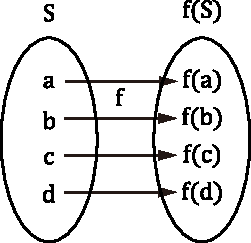
\includegraphics[width = 0.3\linewidth]{./images/image.pdf}
\end{figure}


\paragraph{例}
$ f(x) = x^2 $, 则 $ f(\set{-1, 0, 1, 2}) = \set{0, 1, 4} $.


\begin{definition}[\text{集合的像}]
    $ f \colon X \to Y $ 是一个函数, $ S \subseteq X $. 集合 \[ f(S) = \set{f(x) \colon x \in S} \] 为 $ Y $ 的子集, 称为 $ S $ 在映射 $ f $ 之下的像 (image), 也可称为前像 (forward image).
\end{definition}

简单地说, 像就是经 $ f $ 映射所得到的. 注意, 对单个元素和函数我们也可以有像的概念, 如 $ f(x) = 2x + 1 $, 那么定义域中的元素 $ 1 $ 经过 $ f $ 得到 $ f(1) = 3 $. 于是称陪域中的元素 $ 3 $ 是定义域中的元素 $ 1 $ 的像. 而对于函数, 我们称 $ f $ 的像是 $ f $ 的定义域.

\begin{proposition}
    若 $ x \in S $, 则 $ f(x) \in f(S) $.
\end{proposition}

\begin{proposition}
    设 $ f \colon X \to Y $, $ S \subseteq X $, 则 $ f(S) \subseteq Y $.
\end{proposition}

\begin{proposition}[\text{限制陪域制造双射}]
    设 $ f \colon X \to Y $ 是单射. 按照定义, 如果我们将陪域限制到定义域的像上, 那么 $ f $ 就变成了一个满射, 也就成为了双射. 即 $ \widetilde{f} \colon X \to f(X) $, $ \widetilde{f}(x) = f(x) $ 是一个双射.
\end{proposition}

\begin{remark}
    上面命题的逆命题不再为真. 即 $ f(x) \in f(S) \centernot \Longrightarrow x \in S $. 可以举出反例: $ f(x) = x^2 $, $ f(\set{-1, 0, 1, 2}) = \set{0, 1, 4} $, 有 $ f(-2) \in f(\set{-1, 0, 1, 2}) $, 但 $ -2 \not\in \set{-1, 0, 1, 2} $.
\end{remark}

\begin{definition}[\text{逆像}]
    设函数 $ f \colon X \to Y $. 若 $ U \subseteq Y $, 定义 $ f^{-1} (U) $ 为集合 \[ f ^{-1} (U) \coloneqq \set{x \in X \colon f(x) \in U} \,.\]
    换句话说, $ f^{-1}(U) $ 由 $ X $ 中所有映入 $ U $ 中的元素组成: \[ f(x) \in U \Longleftrightarrow x \in f^{-1}(U) \,.\] $ f^{-1}(U) $ 称为 $ U $ 在 $ f $ 下的逆像 (inverse image), 或称为后像 (backward image).
\end{definition}

$ f $ 和 $ f^{-1} $ 可以看作是两套不同的映射规则, 比如 $ f $ 是加倍, 则 $ f^{-1} $ 是减半, 但这不代表像和逆像是互逆的: $ (f \circ f^{-1})(x) = x $, 见下面的例题. 上面提到 $ f(x) = 2 x + 1 $, $ f(1) = 3 $, 定义域中 $ 1 $ 的像为到达域中的 $ 3 $. 那么与之对应地, $ 1 $ 就是 $ 3 $ 的逆像. 同样的, 逆像也可以指代单个元素和函数.

\begin{remark}
    为了区分像/逆像和函数/反函数, 有时会见到使用方括号表示像或逆像的记号, 如 $ f[S] $ 和 $ f^{-1}[U] $.
\end{remark}

\begin{remark}
    函数的逆和像的逆是两个不同的定义, 尽管它们都有 $ f^{-1} $ 的记号.
\end{remark}

\begin{remark}[\text{等价定义}]
    $ f \colon X \to Y $, 则像可以看成 $ f \colon \cal P (X) \to \cal P (Y) $ 的函数, 逆像可以看成 $ f^{-1} \colon \cal P(Y) \to \cal P(X) $ 的函数. $ \cal P(X) $ 代表 $ X $ 的幂集, 即 $ X $ 所有子集构成的集合.
\end{remark}

\paragraph{例}
$ f \colon \N \to \N $, $ f(x) = 2x $. 那么对于集合 $ \set{1, 2, 3} $ 有 $ f(\set{1, 2, 3}) = \set{2, 4, 6} $. 而 $ f^{-1} (\set{1, 2, 3}) = \set{1} $. 用下面的表示方法可以看出为何像和逆像有前像和后像的别名:
\[ \underset{\text{后像}}{\set{1}} \xlongleftarrow{f^{-1}} \set{1, 2, 3} \xlongrightarrow{f} \underset{\text{前像}}{\set{2, 4, 6}} \,.\]

同时可以注意到, $ f \big( f^{-1}(\set{1, 2, 3}) \big) \neq \set{1, 2, 3} $. $ \set{1, 2, 3} $ 在应用 $ f^{-1} $ 时, 得到的 $ 0.5 $ 和 $ 1.5 $ 不在自然数集中; 再次应用 $ f $ 就无法将这两个数映回到 $ \set{1, 2, 3} $ 中 (因为 $ f $ 的定义域为 $ \N $), 所以 $ f(f^{-1}\set{1, 2, 3}) $ 变小了. 相关命题可见下面的命题.

\begin{proposition}
    对于 $ f \colon X \to Y $ 和 $ f^{-1} $. 设 $ U \subseteq Y $, 则有 $ f \big( f^{-1}(U) \big) \subseteq U $.
\end{proposition}

\begin{proof}
    记 $ S = f^{-1} (U) = \set{x \in X \colon f(x) \in U} $. 所以对任意 $ x \in S \Longrightarrow f(x) \in U $. 设 $ y \in f(S) $, 则 $ y \in \set{f(i) \colon i \in S} $, 而对每个 $ i \in S $, $ f(i) \in U $, 所以 $ y \in U $. 这证明了 $ f(S) \subseteq U $.
\end{proof}

\begin{proposition}
    对于 $ f \colon X \to Y $ 和 $ f^{-1} $. 设 $ S \subseteq X $, 则有 $ f^{-1} \big( f (S) \big) \supseteq S $.
\end{proposition}


\subsection{值域}
有了像的概念就很能引出我们熟知的值域定义.
\begin{definition}[\text{值域}]
    $ f \colon X \to Y $, 则 $ f(x) $ 的值域被定义为 $ X $ 的像, 记作 $ R_f $: \[ R_f = f(X) = \set{f(x) \mid x \in X} \,.\]
\end{definition}

可以看出 $ R_f \subseteq Y $, 也即值域是陪域的子集, 表示陪域中函数能够映射到的元素集合. 



\section{幂集}
\begin{axiom}[\text{幂集公理}]
    设 $ X $, $ Y $ 为集合, 则存在一个集合 $ Y^X $ 表示从 $ X $ 到 $ Y $ 的所有函数的集合. 即: \[ f \in Y^X \Longleftrightarrow \text{$ f $ 是以 $ X $ 为定义域, $ Y $ 为陪域的函数} \,.\]
\end{axiom}

\paragraph{例}
$ X = \set{a, b} $, $ Y = \set{0, 1} $, 则 $ Y^X $ 中有四个函数:
\[ 
    \begin{array}{c}
        f_1 : a \mapsto 0, b \mapsto 0, \\
        f_2 : a \mapsto 0, b \mapsto 1, \\
        f_3 : a \mapsto 1, b \mapsto 0, \\
        f_4 : a \mapsto 1, b \mapsto 1. \\
    \end{array}
\]

\begin{definition}[\text{幂集}]
    设 $ S $ 是集合, 则 $ S $ 的幂集为 $ S $ 所有子集的集合, 记作 $ \cal P (S) $ 或 $ 2^S $: \[ \cal P (S) \coloneqq \set{A \colon A \subseteq S} \,.\]
\end{definition}

$ S $ 中包含的元素数量记作 $ |S| $, $ S $ 的幂集元素数量 $ |\cal P(S)| = 2^{|S|} $, 这即 $ 2^S $ 记号的来源.

\paragraph{例}
$ S = \set{a, b, c} $, 则 $ \cal P(S) = 2^S = \set{\varnothing, \set{a}, \set{b}, \set{c}, \set{a, b}, \set{b, c}, \set{c, a}, \set{a, b, c}} $.


\begin{axiom}
    设 $ A $ 是一个集合, $ A $ 中所有元素都是一个集合. 也就是说 $ A $ 是集合的集合. 则定义 $ A $ 的并: $ \bigcup A $ 为其中每一个元素的并: \[ x \in \bigcup A \Longleftrightarrow \text{对于 $ A $ 中的某个 $ S $, $ x \in S $} \,.\]
\end{axiom}

\paragraph{例}
$ A = \set{\set{1, 2}, \set{2, 3}, \set{3, 4}} $, 则 $ \bigcup A = \set{1, 2, 3, 4} $.

通常我们会给 $ A $ 中的集合加上下标, 给定任意集合 $ I $, 使用其中的元素 $ \alpha \in I $ 给 $ A $ 中的集合标号 $ A_\alpha $. 因此我们称 $ I $ 为指标集, $ \alpha $ 是一个下标或者标签, 所有 $ A_\alpha $ 构成一个集合的族 (简称集族). 比如 $ I = {1, 2, 3} $, $ A $ 中的元素就可以标号为 $ A = \set{A_1, A_2, A_3} $. 于是类似于求和记号, 我们也有记号:
\[ \bigcup_{\alpha \in I} A_\alpha \coloneqq \bigcup \set{A_\alpha \colon \alpha \in I} \,.\]

\begin{remark}
    若 $ I = \varnothing $, $ \displaystyle \bigcup_{\alpha \in I} A_\alpha = \varnothing $.
\end{remark}

\paragraph{例}
$ I = \set{1, 2, 3} $, $ A = \set{A_1, A_2, A_3} $. 则 $ \bigcup A = \bigcup_{\alpha \in I} A_\alpha = A_1 \cup A_2 \cup A_3 $

类比求和, 我们定义类似的记号: \[ \bigcup_{i = 1}^n A_i = A_1 \cup A_2 \cup \cdots \cup A_n \,.\]

\section{笛卡尔积}
\subsection{定义}
\begin{definition}[\text{$ n $-元组}]
    一个 $ n $-元组是由 $ n $ 个对象按照一定次序 $ x_1, x_2, \dots, x_n $ 形成的组, 常记作 $ (x_1, x_2, \dots, x_n) $ 或 $ (x_i)_{1 \leqslant i \leqslant n} $. 规定 $ x_i $ 是第 $ i $ 个分量. 两个 $ n $-元组 $ (x_1, \dots, x_n) $, $ (y_1, \dots, y_n) $ 相等, 当且仅当各分量对应相等: 即 $ 1 \leqslant i \leqslant n $ 时, $ x_i = y_i $.
\end{definition}

$ n $-元组是有序的, 不同于集合. 一个二元组(也称``序偶'') $ (x, y) $ 是不等同于 $ (y, x) $ 的.

\begin{remark}
    一元组 $ (a) $ 和 $ a $ 严格地说是不同的, 但我们不做区分, 将 $ (a) $ 等价于 $ a $.
\end{remark}

\begin{definition}[\text{笛卡尔积}]
    $ X $, $ Y $ 是集合. 则 $ X $ 和 $ Y $ 的笛卡尔积 $ X \times Y $ 定义为: \[ X \times Y \coloneqq \set{(x, y) \mid x \in X, y \in Y} \,.\]
\end{definition}

即从 $ X $ 中拿出一个元素作为第 $ 1 $ 个分量, 从 $ Y $ 中拿出一个元素作为第 $ 2 $ 个分量, 由此构成一个二元组(序偶). $ X $ 和 $ Y $ 构成的所有二元组的集合就是 $ X $ 和 $ Y $ 的笛卡尔积

\paragraph{例}
$ A = \set{a, b, c} $, $ B = \set{0, 1} $, 则 $ A \times B = \set{(a, 0), (a, 1), (b, 0), (b, 1), (c, 0), (c, 1)} $, 而 $ B \times A = \set{(0, a), (0, b), (0, c), (1, a), (1, b), (1, c)} $.

一个多元函数可以看成多个变量, 也可以看成一个变量---输入一个多元组. 如加法函数 $ + \colon \N \times \N \to \N $, $ x + y $ 可以看成变量 $ x $ 和 $ y $ 的二元函数: 输入 $ x $ 和 $ y $, 映射到一个自然数 $ x + y $. 也可以看成 $ (x, y) \mapsto x + y $ 的一元函数: 输入一个二元组 $ (x, y) $, 映射到 $ x + y $.

\begin{proposition}
    $ \varnothing \times A = \varnothing $, $ A \times \varnothing = \varnothing $.
\end{proposition}

\begin{proof}
    假设 $ \varnothing \times A \neq \varnothing $, 即 $ \varnothing \times A $ 非空, 那么可以从中取出一个元素 $ (x, y) $, 按照定义, $ x $ 和 $ y $ 满足 $ x \in \varnothing $, $ y \in A $. 而不存在 $ x \in \varnothing $, 这产生了矛盾. 所以 $ \varnothing \times A = \varnothing $. 同理也可以证明 $ A \times \varnothing = \varnothing $.
\end{proof}


\subsection{多重笛卡尔积}
笛卡尔积可以推广到 $ n $ 重:
\begin{definition}[\text{$ n $ 重笛卡儿积}]
    \[ \prod_{i = 1}^n X_i = X_1 \times X_2 \times \cdots \times X_n \coloneqq \set{(x_i)_{1 \leqslant i \leqslant n} \mid x_i \in X_i } \,.\]
\end{definition}

\begin{remark}
    严格地说, $ X \times Y \times Z \neq (X \times Y) \times Z \neq X \times (Y \times Z) $. 但由于三者间互相存在双射关系, 故常常不做区分, 看作是一样的.
\end{remark}

\begin{remark}
    空的笛卡尔积给出单元素集, 如 $ \prod_{1 \leqslant i \leqslant 0} X_i = \set{()} $, 里面的元素为空组 $ () $. 
\end{remark}

\begin{remark}
    $ \prod_{i = 1}^n X = X \times X \times \cdots \times X = X^n $. 这个记法就是 $ \R^2 $, $ \R^3 $, $ \R^n $ 等记号来源.
\end{remark}

和前面一样, $ f \colon X \times Y \times Z \to W $, 既可以看作是 $ X \times Y \times Z $ 的一元函数, 也可以看作 $ X $ 和 $ Y \times Z $ 的二元函数, 还可以看作 $ X $, $ Y $, $ Z $ 上的三元函数. 也不作区分.

下面推广单个选择公理到有限多个选择, 随后还能推广到无限个的情况.
\begin{lemma}[\text{有限选择}]
    设 $ X_i $, $ 1 \leqslant i \leqslant n $ 是一系列非空集合. 则存在多元组 $ (x_i)_{1 \leqslant i \leqslant n} $, 使得对一切 $ 1 \leqslant i \leqslant n $, $ x_i \in X_i $. 这等价于: 若 $ X_i $ 非空, 则 $ \displaystyle \prod_{1 \leqslant i \leqslant n} X_i $ 非空. 
\end{lemma}

换句话说, 如果 $ X_1, X_2, \dots, X_n $ 都是非空的, 则可以分别从中选出元素 $ x_i \in X_i $, 构成一个多元组 $ (x_1, x_2, \dots, x_n) $, 以证明这一点.

这个引理可以通过归纳法证明. 


\section{基数}
\subsection{基数定义}
\begin{definition}[\text{非正式}]
    基数为集合中元素的个数. 我们用自然数来清点集合中的元素.
\end{definition}

基数描述了集合的大小(元素多少). 

\begin{definition}[\text{基数相同}]
    我们称集合 $ A $ 和 $ B $ 的基数相同, 当且仅当 $ A $ 和 $ B $ 之间存在双射 $ f \colon A \to B $.
\end{definition}

\paragraph{例}
$ \set{1, 2, 3} $ 和 $ \set{4, 5, 6} $ 的基数是相同的. 因为存在一种双射 $ 1 \leftrightarrow 4 $, $ 2 \leftrightarrow 5 $, $ 3 \leftrightarrow 6 $.

\begin{proposition}[\text{基数相同是一种等价关系}]
    \ 
    \begin{enumerate}
        \item 自反: $ A $ 和 $ A $ 基数相同
        \item 对称: $ A $ 和 $ B $ 的基数相同, 则 $ B $ 和 $ A $ 的基数相同
        \item 传递: $ A $ 和 $ B $ 的基数相同, $ B $ 和 $ C $ 的基数相同, 则 $ A $ 和 $ C $ 的基数相同
    \end{enumerate}
\end{proposition}

\begin{definition}[\text{基数}]
    设 $ n $ 为自然数. $ X $ 的基数为 $ n $, 当且仅当它与 $ \set{i \in \N \mid 1 \leqslant i \leqslant n} $ 有相同的基数. $ X $ 有 $ n $ 个元素, 当且仅当其基数为 $ n $, 记作 $ |X| = n $.
\end{definition}

\begin{remark}
    可以用 $ \set{i \in \N \colon i < n} $ 代替 $ \set{i \in \N \colon 1 \leqslant i \leqslant n} $, 因为它们的基数相同.
\end{remark}

\begin{remark}
    当 $ n = 0 $, $ \set{i \in \N \colon 1 \leqslant i \leqslant 0} $ 为空集. 说明空集的基数为 $ 0 $.
\end{remark}

\paragraph{例}
$ \set{a, b, c} $ 和 $ \set{i \in \N \colon 1 \leqslant i \leqslant 3} = \set{1, 2, 3} $ 有相同的基数 $ 3 $.

$ \set{-1, 0, 1, 2} $ 和 $ \set{i \in \N \colon i < 4} = \set{0, 1, 2, 3} $ 有相同的基数 $ 4 $.

\begin{proposition}[\text{基数的唯一性}]
    对于任意基数为 $ n $ 的集合 $ X $, 若 $ m \neq n $, 则 $ X $ 的基数必然不是 $ m $.
\end{proposition}

\begin{lemma} \label{cardinary}
    若非空集合 $ X $ 的基数为 $ n $, 显然 $ n \geqslant 1 $. 现从 $ X $ 中选出一个元素 $ x $, 则 $ X \setminus \set x $ 的基数为 $ n - 1 $.
\end{lemma}

证明思路不难理解, $ X $ 和 $ \set{i \in \N \colon 1 \leqslant i \leqslant n} $ 存在一个双射 $ f $. 当我们从 $ X $ 中剔除掉 $ x $ 元素后, 原来 $ x $ 对应的 $ f(x) $ 也没有对应元素了. 我们将原本到 $ f(x) $ 后面元素的映射向前挪一个位置, 就能形成一个基数为 $ n - 1 $ 的双射了. 

\begin{proof}[\text{证明引理}]
    设 $ f \colon X \to \set{i \in \N \colon 1 \leqslant i \leqslant n} $, $ f $ 应为双射. 现在去除 $ x $ 元素后, 构造一个新映射 $ g \colon X \setminus \set x \to \set{i \in \N \colon 1 \leqslant i \leqslant n - 1} $. 由于 $ f $ 是双射, 对于 $ y \in X \setminus \set x $, $ f(y) \neq f(x) $. 当 $ f(y) < f(x) $ 时, $ g(y) = f(y) $; 当 $ f(y) > f(x) $ 时, $ g(y) = f(y) - 1 $. 接下来只要验证 $ g $ 为双射, 引理就得到证明. 
    
    先验证 $ g $ 为单射: 取集合 $ X \set{x} $ 中任意的不同 $ a $, $ b $. 因为 $ a \neq b $, $ f $ 为双射, 所以 $ f(a) \neq f(b) $. $ f(a) $, $ f(b) $ 和 $ f(x) $ 共有 $ 4 $ 种关系: $ f(a), f(b) $ 同大于/小于 $ f(x) $, $ f(a), f(b) $ 一个大于 $ f(x) $ 一个小于 $ f(x) $. 先看前一种 $ f(a) > f(x) $, $ f(b) > f(x) $, 则 $ g(a) = f(a) - 1 $, $ g(b) = f(b) - 1 $. 由于前面推出了 $ f(a) \neq f(b) $, $ g(a) \neq g(b) $. 同小于 $ f(x) $ 的情况同理. 下面看 $ f(a), f(b) $ 一个大于一个小于 $ f(x) $. 设 $ f(a) > f(x) > f(b) $, $ g(a) = f(a) - 1 $, $ g(b) = f(b) $. $ f(b) < f(x) < f(a) \Longrightarrow f(b) + 1 \leqslant f(x) < f(a) \Longrightarrow f(b) + 1 \neq f(a) $, 故 $ g(a) \neq g(b) $. $ f(b) > f(x) > f(a) $ 情况同理. 以上说明 $ g $ 是单射.

    再验证 $ g $ 是满射: 对于所有 $ f(x) \leqslant y \leqslant n - 1 $ 时, $ \exists s \in X \setminus \set x $, 使得 $ g(s) = f(s) - 1 = y $. 对于所有 $ 1 \leqslant y < f(x) $, $ \exists s \in X \setminus \set x $, 使得 $ g(s) = f(s) = y $. 即满射.
\end{proof}


\begin{proof}[\text{证明基数的唯一性}]
    假设 $ X $ 为空集, 基础情形满足. 现设对含有 $ n $ 个元素的 $ X $, 命题成立. 要证明 $ X $ 基数为 $ n + 1 $ 时命题成立. 应用反证法, 假设对基数 $ n + 1 $ 的 $ X $, 存在 $ m \neq n + 1 $ 使得 $ X $ 的基数也为 $ m $. 那么根据引理, 从非空的 $ X $ 中选择出一个元素 $ x $, 集合 $ X \setminus \set{x} $ 的基数为 $ m - 1 $, 同时有基数为 $ n $. 那么根据归纳假设, $ m - 1 = n $, 即 $ m = n + 1 $. 这与 $ m \neq n + 1 $ 矛盾. 所以 $ m = n + 1 $, 而这完成了归纳.
\end{proof}


\subsection{有限集与无限集}
\begin{definition}[\text{有限集}]
    一个集合是有限的, 当且仅当它的基数是某个自然数 $ n $; 否则集合称为无限的. 如果 $ X $ 是有限集, $ |X| $ 表示其基数.
\end{definition}

\paragraph{例}
$ |\set{0, 1, 2, 3}| = 4 $, $ |\set{i \in \N \colon 2 \leqslant i \leqslant 4}| = 3 $, $ |\varnothing| = 0 $.

\begin{lemma}[\text{有限序列有界}]
    设存在有限序列 $ a_1, a_2, \dots, a_n $, $ n \in \Z^+ $, 则这个序列是有界的.
\end{lemma}

\begin{proof}
    当 $ n = 1 $ 时, 序列只有一项 $ a_1 $. 显然能够找到 $ M_1 \in \R $ 使得 $ |a_1| \leqslant M_1 $. 这证明了基础情形. 现假设 $ a_1, a_2, \dots, a_n $ 是有界的, 要证明 $ a_1, a_2, \dots, a_{n + 1} $ 也是有界的.

    设对所有 $ 1 \leqslant i \leqslant n $ 有 $ |a_i| \leqslant M $. 取 $ M' = M + |a_{n + 1}| $, 则有 $ |a_i| \leqslant M' $, 同时有 $ |a_{n + 1}| \leqslant M' $. 故 $ |a_i| \leqslant M' $ 对一切 $ 1 \leqslant i \leqslant n+1 $ 成立, 即 $ a_1, a_2, \dots, a_{n + 1} $ 有界, 而这完成了归纳.
\end{proof}


\begin{theorem}
    自然数 $ \N $ 是无限集.
\end{theorem}

\begin{proof}
    假设 $ \N $ 是有限集. 则存在自然数 $ n $, 以及双射 $ f \colon \set{i \in \N \colon 1 \leqslant i \leqslant n} \to \N $. 考虑序列 $ f(1), f(2), \dots, f(n) $. 这个序列是有限的, 则也是有界的. 那么存在 $ M \in \N $, 使得 $ |f(i)| \leqslant M $ 对一切 $ 1 \leqslant i \leqslant n $ 成立. 考虑陪域中的 $ M + 1 \in \N $, 在定义域中没有对应元素 $ x \in \set{i \in \N \colon 1 \leqslant i \leqslant n} $ 使得 $ f(x) = M + 1 $, 这和 $ f $ 双射的假设矛盾. 所以 $ \N $ 不是有限集, 也就是无限集.
\end{proof}

\subsection{基数性质}
下面着重讲解有限集上的基数性质.

\begin{lemma}[\text{子集-单射存在}] \label{subset-injection}
    $ X \subseteq Y $ 则存在单射 $ f \colon X \to Y $.
\end{lemma}

\begin{proof}
    对于 $ X \subseteq Y $, 考虑映射 $ f\colon X \to Y $, $ f(x) = x $. 考虑 $ x, y \in X $ 且 $ x \neq y $, 则有 $ x = f(x) $ 和 $ y = f(y) $, 于是 $ f(x) \neq f(y) $, 即 $ f $ 为单射.
\end{proof}

\begin{proposition}[\text{有限集上的基数性质}] \label{cardinal II}
    设 $ X $, $ Y $ 均为有限集.
    \begin{enumerate}
        \item $ x \notin X $, 则 $ X \cup \set{x} $ 也为有限集, 且 $ |X \cup \set{x}| = |X| + 1 $
        \item $ |X \cup Y| \leqslant |X| + |Y| $. 若 $ X $, $ Y $ 互斥, 即 $ X \cap Y = \varnothing $, 则 $ |X \cup Y| = |X| + |Y| $
        \item (子集-基数) $ X \subseteq Y $ 则 $ |X| \leqslant |Y| $. 而如果 $ X $ 是 $ Y $ 的真子集, 即 $ X \neq Y $, 则 $ |X| < |Y| $
        \item (单射-基数) 存在单射 $ f\colon X \to Y $ 当且仅当 $ |X| \leqslant |Y| $, 两者是等价关系.
        \item (像的缩小) 函数 $ f \colon X \to Y $. 有 $ |f(X)| \leqslant |X| $. 若 $ f $ 是单射, 则 $ |f(X)| = |X| $
        \item $ |X \times Y| = |X| \times |Y| $
        \item $ |Y^X| = |Y|^{|X|} $
    \end{enumerate}
\end{proposition}

有限集中, 子集-单射-基数三者的关系可以表示如下:
\begin{figure}[H]
    \centering
    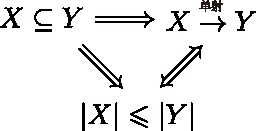
\includegraphics[width = 0.35\linewidth]{./images/implies.pdf}
\end{figure}


\begin{proof}
    (1) 由引理 \ref{cardinary}, $ |X \cup \set{x} \setminus \set{x}| = |X| = |X \cup \set{x}| - 1 $. 所以 $ |X \cup \set{x}| = |X| + 1 $.

    (2) 设 $ |X| = n $, $ |Y| = m $. 则存在双射 $ f \colon X \to \colon \set{i \in \N \colon 1 \leqslant i \leqslant n} $ 和双射 $ g \colon Y \to \set{i \in \N \colon 1 \leqslant i \leqslant m} $. 现定义函数 $ h \colon X \cup Y \to \set{i \in \N \colon 1 \leqslant i \leqslant m + n} $.
    \[ h(x) = \begin{cases}
        f(x) & x \in X \\
        g(x) + n & x \in Y, x \notin X
    \end{cases} \]

    下面证明 $ h $ 是单射: 对于不同的 $ x, y \in X \cup Y $, 我们可以不失一般性地分类讨论三种情况. (i) 当 $ x, y \in X $: 那么 $ h(x) = f(x) $, $ h(y) = f(y) $. 由于 $ f $ 是双射, $ f(x) \neq f(y) $, 所以 $ h(x) \neq f(y) $. (ii) 当 $ x \in X $, $ y \in Y $ 且 $ y \notin X $: $ h(x) = f(x) $, $ h(y) = g(y) + n $. 由于 $ 1 \leqslant f(x) \leqslant n $, $ n + 1 \leqslant g(x) + n \leqslant n + m $, 所以有 $ h(x) \neq h(y) $. (iii) 当 $ x, y \in Y $ 且 $ x, y \notin X $: $ h(x) = g(x) + n $, $ h(y) = g(y) + n $. 而因为双射已经有 $ g(x) \neq g(y) $, 故 $ h(x) \neq h(y) $. 综上所述, $ h $ 为单射.

    当 $ X $, $ Y $ 互斥, 即 $ X \cap Y = \varnothing $. 对于每一个 $ 1 \leqslant i \leqslant n $, 能找到对应的 $ x \in X $, 满足 $ i = h(x) = f(x) $; 而对于每一个 $ n + 1 \leqslant j \leqslant m + n $, 能找到对应 $ y \in Y $, 满足 $ j = h(y) = g(y) + n $. 所以 $ h $ 是满射.

    当 $ X $, $ Y $ 不互斥, $ X \cap Y \neq \varnothing $. 考虑 $ x \in X \cap Y $, $ g(x) + n \in \set{i \in \N \colon 1 \leqslant i \leqslant m + n} $. 一方面: 对于一切 $ y \in X $, $ h(y) = f(y) $, $ 1 \leqslant f(y) \leqslant n $, $ n + 1 \leqslant g(x) + n \leqslant m + n $, 所以找不到 $ y \in X $, 满足 $ h(y) = g(x) + n $. 另一方面: 对于一切 $ y \in Y $ 但 $ y \notin X $, $ x \neq y $, $ h(y) = g(y) + n \neq g(x) + n $ (因为 $ g $ 是双射), 所以找不到 $ y \in Y $ 且 $ y \notin X $ 满足 $ h(y) = g(x) + n $. 综上所述, 找不到 $ y \in X \cup Y $, 满足 $ h(y) = g(x) + n $. 这说明 $ h $ 不是满射.

    于是综上所述, 当 $ X $, $ Y $ 互斥时, $ h \colon X \cup Y \to \set{i \in \N \colon 1 \leqslant i \leqslant m + n} $ 是双射: $ |X \cup Y| = m + n = |X| + |Y| $. 
    
    而当 $ X $, $ Y $ 不互斥时, $ h $ 仅为单射, 通过限制陪域, 构造 $ \widetilde{h} \colon X \cup Y \to h(X \cup Y) $, $ \widetilde{h} (x) = h(x) $. $ \widetilde{h} $ 是一个双射, 故 $ |X \cup Y| = |h(X \cup Y)| $. 并且 $ h(X \cup Y) \subseteq \set{i \in \N \colon 1 \leqslant i \leqslant m + n} $. 不妨记 $ H = h(X \cup Y) $, $ I = \set{i \in \N \colon 1 \leqslant i \leqslant m + n} $, $ H \subseteq I $. $ I = (I \setminus H) \cup H $, 且 $ I \setminus H $ 和 $ H $ 是互斥的. 所以 $ |I| = |I \setminus H| + |H| $, 即 $ |H| \leqslant |I| $. 所以最终, $ |X \cup Y| = |h(X \cup Y)| \leqslant |I| = m + n = |X| + |Y| $.

    (3) $ X \subseteq Y $, 则 $ Y = X \cup (Y \setminus X) $ 以及 $ X \cap (Y \setminus X) = \varnothing $. 于是由 (2) 有 $ |Y| = |X \cup (Y \setminus X)| = |X| + |Y \setminus X| \geqslant |X| $. 若 $ X \subset Y $, 存在 $ a \in Y $ 但 $ a \notin X $. 对于每一个 $ b \in X $, $ b \in Y $, $ a \neq b $. 所以 $ b \in Y \setminus \set{a} $, 所以 $ X \subseteq Y \setminus \set{a} $. 所以 $ |X| \leqslant |Y - \set{a}| = |Y| - 1 $, 则 $ |X| < |Y| $.

    (4) 单射 $ \Longrightarrow |X| \leqslant |Y| $: 反证法. 设存在单射 $ f \colon X \to Y $ 且 $ |X| > |Y| $. 那么设 $ |X| = n $, $ |Y| = m $, $ n > m $. 按照基数的定义, 存在双射 $ g \colon \set{i \in \N \colon 1 \leqslant i \leqslant n} \to X $ 以及 $ h \colon Y \to \set{i \in \N \colon 1 \leqslant i \leqslant m} $. 由命题 \ref{c}: 单射的复合仍为单射. 于是 $ h \circ f \circ g \colon \set{i \in \N \colon 1 \leqslant i \leqslant n} \to \set{i \in \N \colon 1 \leqslant i \leqslant m} $ 仍为单射. 注意到 $ \forall x \in \set{i \in \N \colon 1 \leqslant i \leqslant m} $, $ x \in \set{i \in \N \colon 1 \leqslant i \leqslant n} $, 故 $ \set{i \in \N \colon 1 \leqslant i \leqslant m} \subseteq \set{i \in \N \colon 1 \leqslant i \leqslant n} $. 由 (3): $ |\set{i \in \N \colon 1 \leqslant i \leqslant m}| \leqslant |\set{i \in \N \colon 1 \leqslant i \leqslant n}| $, 即 $ m \leqslant n $, 这与 $ n > m $ 矛盾.

    $ |X| \leqslant |Y| \Longrightarrow $ 单射: 记 $ I_{k} = \set{i \in \N \colon 1 \leqslant i \leqslant k} $. 同样设 $ |X| = n $, $ |Y| = m $, $ n \leqslant m $. 存在双射 $ f \colon X \to I_n $ 以及 $ g \colon Y \to I_m $. 可知 $ I_n \subseteq I_m $. 所以由引理 \ref{subset-injection}, 存在单射 $ h \colon I_n \to I_m $. 我们重新组织 $ f $, $ g $, $ h $ 的关系 (注意 $ Y $ 到 $ I_m $ 有双射, $ I_m $ 到 $ Y $ 也有双射): \[ X \xlongrightarrow{f} I_n \xlongrightarrow{h} I_m \xlongrightarrow{g} Y \,.\]

    那么存在 $ X $ 到 $ Y $ 的映射 $ g \circ h \circ f $, 且其为单射 (单射的复合仍为单射).
\end{proof}


\section{无限集合}


\end{document}